%%%% 
% This is a template for project reports in the subject DAT620 at the
% Department of Electrical Engineering and Computer Science,
% University of Stavanger.
% 
% The template is based on the ACM conference template 
% it was edited by Leander Jehl and Hein Meling
\documentclass[sigconf]{acmart}

%DON'T CHANGE THIS FILE
%This file sets several properties for the ACM template.
%It is not necessary to change this file.


% Copyright
\setcopyright{none}

% DOI
\acmDOI{}

% ISBN
\acmISBN{}

%Conference
\acmConference[Project in Computer Science (DAT500)]{}{IDE}{UiS}
\acmBooktitle{}
\copyrightyear{2023}

\newcommand{\supervisors}[1]{\thanks{Supervised by #1}}


%In the preamble file you can include packages and define macros.
\usepackage{xspace}

%Here we define a marco: The \xspace ensures correct spacing, i.e. insert space before next word, but not before period or comma.
\newcommand{\paxos}{\textsc{Paxos}\xspace}

%These packages are needed for the plot in Figure 1. 
\usepackage{tikz}
\usepackage{pgfplots}
\pgfplotsset{compat=newest}

\usepackage{hyperref}
\hypersetup{
    colorlinks=true,
    linkcolor=blue,
    filecolor=magenta,      
    urlcolor=cyan,
    pdftitle={Overleaf Example},
    pdfpagemode=FullScreen,
}
\urlstyle{same}

\usepackage{listings}
\usepackage{color}
\usepackage{tikz}
\usepackage[utf8]{inputenc}

\DeclareFixedFont{\ttb}{T1}{txtt}{bx}{n}{12}
\DeclareFixedFont{\ttm}{T1}{txtt}{m}{n}{12}

\definecolor{codegreen}{rgb}{0,0.6,0}
\definecolor{codegray}{rgb}{0.5,0.5,0.5}
\definecolor{codepurple}{rgb}{0.58,0,0.82}
\definecolor{backcolour}{rgb}{0.95,0.95,0.9}
\definecolor{deepblue}{rgb}{0,0,0.5}
\definecolor{deepred}{rgb}{0.6,0,0}
\definecolor{deepgreen}{rgb}{0,0.5,0}
\definecolor{uislight}{HTML}{0a3c9f}
\definecolor{uisdark}{HTML}{0a3ca0}
\definecolor{uisorange}{HTML}{ff9e3d}
\definecolor{uisgrey}{HTML}{e1e1e1}

\lstdefinestyle{mystyle}{
    language=Python,
    basicstyle=\ttfamily\tiny,
    morekeywords={self},
    keywordstyle=\ttb\color{deepblue},
    emph={MyClass,__init__},
    emphstyle=\ttb\color{deepred},
    stringstyle=\color{deepgreen},
    frame=tb,
    showstringspaces=false
    commentstyle=\color{codegreen},
    keywordstyle=\color{magenta},
    numberstyle=\tiny\color{codegray},
    stringstyle=\color{codepurple},
    breakatwhitespace=false,         
    breaklines=true,                 
    captionpos=b,                    
    keepspaces=true,                 
    numbers=left,                    
    numbersep=4pt,                  
    showspaces=false,                
    showstringspaces=false,
    showtabs=false,                  
    tabsize=1
}
\lstset{style=mystyle}

\counterwithin{figure}{section}
\counterwithin{table}{section}



\begin{document}
%TODO: Replace the title with your project title.
\title{Flight Delay Trends}
%you may use a subtitle
\subtitle{DAT500 project in Spring of 2023}

%TODO replace author names with your name and email below:
\author{Bhakti Prabhu}
\affiliation{University of Stavanger, Norway}
\email{br.prabhu@stud.uis.no}
\author{Stephan Frederik Werner Brandasu}
\affiliation{University of Stavanger, Norway}
\email{sf.brandasu@stud.uis.no}

%TODO: add the name of one or more supervisors
%\supervisors{Rui Paulo Maximo Pereira Mateu Esteves and Jayachander Surbiryala}


\begin{abstract}
%The abstract lies in a different file: 
\textbf{In this paper, we aimed to analyse flight delay and cancellation trends using big data technologies such as Hadoop and Spark. By leveraging data from the U.S. Department of Transportation Statistics, we aimed to identify patterns in the data to answer questions such as which months or weeks have the most delayed or cancelled flights and which carriers are more likely to experience delays.}

The paper focuses mainly on how we utilized Hadoop and Spark technologies, for building the application and the Spark optimisation techniques used to improve the performance of the application. We discuss the different performance problems we faced while executing a Spark application and the measures we took to mitigate some of those issues. Specifically, we discuss the problems of data skew, spill, serialisation and shuffle. For each of these issues, we suggest techniques for optimizing Spark applications, such as data partitioning, optimizing code and choosing appropriate aggregation methods while transforming the data.

Overall, our paper demonstrates the practical use of big data technologies to extract insights from large datasets and highlights the challenges and solutions associated with processing large datasets and optimizing the execution process. The findings of our use case could be useful for travellers, airlines, airport authorities, and other stakeholders in the aviation industry to better understand the causes of flight delays and cancellations and to take appropriate measures to improve their performance.


\end{abstract}

%TODO: Replace with some keywords, relevant for your project
\keywords{flight delay, spark, pyspark, hadoop, spark optimisations}

\maketitle

%Each section can be placed in a separate file and included by the input command.

\section{Introduction}
\label{sec:introduction}
\subsection{Use Case}
Did you ever experience being stranded in an airport because of flight delays or cancellations, and pondered on the possibility of being able to predict it with the help of more data? The use case that we chose for our project poses a solution for this problem. The U.S. Department of Transportation Statistics (DTS) tracks the on-time performance of domestic flights operated by large air carriers\cite{dataset}. Summary information on the number of on-time, delayed, cancelled, and diverted flights is published in the DTS's monthly Air Travel Consumer Report. We have taken our dataset from their official website. The dataset consists of the flight delay and cancellation information for the years from 2018 to 2022.

The goal of our use case is to analyse the trends in delays, to get an understanding of how the flight on-time performance varies in a particular time period. This analysis gives answer to various questions like, during which months in a year flights get most delayed, which day or week in a month has more possibility of flights getting delayed or cancelled, which flight carrier gets delayed more often compared to others and many more similar questions. This information can be useful for both a traveller and the airline carrier. Having access to this information a traveller can ensure that they do not miss any important meetings or events, while at the same time an airline carrier can know when it needs to increase their work force and use this opportunity to improve over their competitors.

\subsection{Background}
The goal of this project is to learn and get understanding of Hadoop and Spark Technologies which are frameworks for handling data intensive systems or nowadays commonly known as Big Data. Apache Hadoop is a collection of open-source modules and utilities intended to make the process of storing, managing and analysing big data easier while Apache Spark is an open-source data processing engine built for efficient, large-scale data analysis. Apache Spark can be run either standalone or as a software package on top of Apache Hadoop.

For our project we used Hadoop for converting our unstructured data which was in Text format to structured Comma Separated Values (.CSV) files. We used MapReduce in Hadoop to achieve this. Next, we used Spark to read this structured file from Hadoop Distributed File System (HDFS) and do the required processing on the dataset in line with the goal of our use case. One of the main aims of our project was to understand spark optimization techniques. We learnt about the five most common performance issues that can be encountered while executing a spark application, those issues are spill, skew, shuffle, storage and serialisation. From those five we selected the 3 which we believed would help the most at making our application run faster. 

\subsection{optimisations}
Among these, we observed that our spark application can be improved by solving problems related to Spill and Skew (Inter-related in our case), Shuffle and Serialization.

\emph{Spill} is the term used to refer to the act of moving an RDD from RAM to disk, and later back into RAM again. This occurs when a given partition is simply too large to fit into RAM. In this case, Spark is forced into potentially expensive disk reads and writes to free up local RAM. All of this just to avoid the dreaded OOM (Out of Memory) Error. One of the reasons of Spill could be the Skew in the dataset. Hence, skew can induce spill. We observed that there was skew in our dataset, there was a lot more information on some carriers compared to very little information on other carriers. We also observed in the Spark UI that there was Spill in some of the stages of execution of the application processes.

\emph{Shuffle} is a side effect of wide transformation caused by operations like join() and group by() on the data. Shuffling refers to transfer of data over the network which adds as overhead time to the actual processing time. Since we are using multiple of these operations in our application, we chose to attempt to minimise this problem.

\emph{Serialization} occurs when the code has to be serialised, this means that the code is sent to the executors and then de-serialised before it can be executed. Python code will take an even harder hit due to it having to be pickled and the spark must initiate an instance of the python interpreter in every single executer. meanwhile Spark SQL and Dataframe instructions are compact and optimized for distribution instructiosn from the driver to each executor. Our code was using a few User Defined Functions (UDF's) so this was the last of our 3 optimisations.



\section{Methods}
\label{sec:methods}
\subsection{Cluster Configuration} 
The resources for implementing and executing the application was provided to us by the University of Stavanger. We had 1 Name node (Master) with 4GB RAM and 2 CPU cores, and 3 Data nodes (workers) with 8GM RAM, 4 CPU cores and 80GB of disk space on each node, which totals out to 24GB RAM, 12 cores and 240GB disk space for parallel processing on data stored in the HDFS using YARN as the resource manager. Our application is built on Apache Hadoop version 3.2.1 and Spark version 3.2.4. Our Spark application is coded in Python language using the Pyspark(3.2.4) APIs. 


\subsection{The Dataset}
We obtained our dataset from the website of the US Department of Transportation Statistics. The data about the On-Time Performance of Flights was available on the site in monthly format, meaning the data was downloaded in a month by month format. We decided to work with 5 years spanning from 2018-2022. The data in its unsorted text form came out to be a total of 20.7GB. How the files were named can be seen in figure \ref{fig:Text_Files_size}.

\begin{figure}[H]
\centering
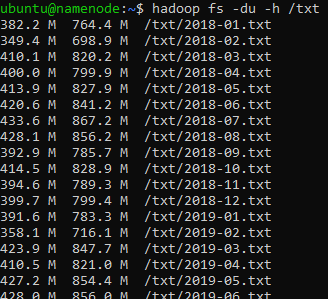
\includegraphics[width=0.30\textwidth]{fig/unstructured_dataset_size.png}
\caption{Truncated view of the file system showing the text files}
\label{fig:Text_Files_size}
\end{figure}

After converting the dataset from text format to CSV using a Map job in Hadoop, the dataset size reduced to 5.9GB having all flight performance attributes in 38 columns. We stored our dataset in CSV format in two ways. First with year by year CSV files, and second all 5 years data in a single CSV file. The idea behind this was that we could easily test the upsert functionality of the delta table using the year by year files while we could test the performance of the application using the larger combined file. The file naming format and sizes can be seen in figure \ref{fig:CSV_Files}.

\begin{figure}[H]
\centering
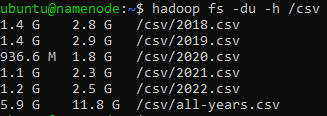
\includegraphics[width=0.30\textwidth]{fig/structured_dataset_size.png}
\caption{view of the file system showing the csv files}
\label{fig:CSV_Files}
\end{figure}


\subsection{Mapping}
The dataset from the start is unstructured as a text document where each field is listed sequentially in a [key, value] format as shown in figure \ref{fig:orig_text_data}. This meant that to ingest the data and structure it as CSV, we went through each row of the text file, cleaning the data of any commas that might exist and extracting the value into a list element. Once the last key for a single row of data was found the list would be printed and we could move on to the next row. \cite{hadoop}

\begin{figure}[H]
\centering
\begin{lstlisting}
YEAR 2022
QUARTER 4
MONTH 12
DAY_OF_MONTH 1
DAY_OF_WEEK 4
FL_DATE 12/1/2022 12:00:00 AM
OP_UNIQUE_CARRIER 9E
TAIL_NUM N131EV
OP_CARRIER_FL_NUM 4736
ORIGIN_AIRPORT_ID 12323
ORIGIN_AIRPORT_SEQ_ID 1232305
ORIGIN_CITY_MARKET_ID 32323
ORIGIN ILM
ORIGIN_CITY_NAME Wilmington, NC
ORIGIN_STATE_NM North Carolina
DEST_AIRPORT_ID 10397
DEST_AIRPORT_SEQ_ID 1039707
DEST_CITY_MARKET_ID 30397
DEST ATL
DEST_CITY_NAME Atlanta, GA
DEST_STATE_NM Georgia
DEP_DELAY 14.00
DEP_DELAY_NEW 14.00
DEP_DEL15 0.00
ARR_DELAY -2.00
ARR_DELAY_NEW 0.00
ARR_DEL15 0.00
CANCELLED 0.00
CANCELLATION_CODE 
DIVERTED 0.00
CARRIER_DELAY 
WEATHER_DELAY 
NAS_DELAY 
SECURITY_DELAY 
LATE_AIRCRAFT_DELAY 
\end{lstlisting}
\caption{The original dataset in text format with a key, value structure}
\label{fig:orig_text_data}
\end{figure}

As can be seen in figure \ref{fig:orig_text_data} not all columns of a row would have data in them. In this case we would return an empty string into the list so that the CSV would stay consistent. Additionally we stripped any commas which might exist in the data to avoid any potential issues in the final CSV.

In figure \ref{fig:mapper} it can be seen how we went through each line of the text file, stripping it of commas, then checking if it is the final column of a data row. 
 
\begin{figure}[H]
\centering
\begin{lstlisting}
import sys

row = []

for line in sys.stdin:
  line = line.strip().replace(',','').split()

  if line[0] == "LATE_AIRCRAFT_DELAY":
    try:
      data = line[1]
    except IndexError:
      data = ' '
    row.append(data)
    print(','.join(row))
    row = []
  else:
    try:
      data = ' '.join(line[1:])
    except IndexError:
      data = ' '
    row.append(data)
\end{lstlisting}
\caption{The Hadoop map script}
\label{fig:mapper}
\end{figure}

Regardless of if the line was the last column or not we had to make sure that the application wouldn't error out due to not finding any value for the key so we inserted either the value or effectively a null into the list before either continuing to build the list, or printing it.

Below in figure \ref{fig:mapper_command} an example of how we read in the text files can be seen. Here we read in all the text files for the year 2022 and merged them into a single output file so that we would be working with less files in Pyspark.

\begin{figure}[H]
\centering
\begin{lstlisting}
mapred streaming -files flight_mapper.py \
-input /txt/2022-12.txt,/txt/2022-11.txt,/txt/2022-10.txt,/txt/2022-09.txt,/txt/2022-08.txt,/txt/2022-07.txt,/txt/2022-06.txt,/txt/2022-05.txt,/txt/2022-04.txt,/txt/2022-03.txt,/txt/2022-02.txt,/txt/2022-01.txt \
-output /csv/2022.csv \
-mapper "flight_mapper.py"
\end{lstlisting}
\caption{the Mapred Command}
\label{fig:mapper_command}
\end{figure}

\subsubsection{The Data Struct}
When reading data into Pyspark we wanted to make sure that it existed in a consistent and logical structure. To do this we made 3 Structs for each type of table which we would read in, these Structs can be seen in fig \ref{fig:structs}. The $flgithschema$ was made to read in all of the data which was created by the Hadoop mapping job. Each field was given the correct type whether that be a string, integer or a float. They were also given their original names from the text file so that we knew what was what.

\begin{figure}[H]
\centering
\begin{lstlisting}
flightSchema = StructType() \
	.add('YEAR', 'integer')\
	.add('QUARTER', 'integer')\
	.add('MONTH', 'integer')\
	.add('DAY_OF_MONTH', 'integer')\
	.add('DAY_OF_WEEK', 'integer')\
	.add('FL_DATE', 'string')\
	.add('OP_UNIQUE_CARRIER', 'string')\
	.add('TAIL_NUM', 'string')\
	.add('OP_CARRIER_FL_NUM', 'integer')\
	.add('ORIGIN_AIRPORT_ID', 'integer')\
	.add('ORIGIN_AIRPORT_SEQ_ID', 'integer')\
	.add('ORIGIN_CITY_MARKET_ID', 'integer')\
	.add('ORIGIN', 'string')\
	.add('ORIGIN_CITY_NAME', 'string')\
	.add('ORIGIN_STATE_NM', 'string')\
	.add('DEST_AIRPORT_ID', 'integer')\
	.add('DEST_AIRPORT_SEQ_ID', 'integer')\
	.add('DEST_CITY_MARKET_ID', 'integer')\
	.add('DEST', 'string')\
	.add('DEST_CITY_NAME', 'string')\
	.add('DEST_STATE_NM', 'string')\
	.add('DEP_DELAY', 'float')\
	.add('DEP_DELAY_NEW', 'float')\
	.add('DEP_DEL15', 'float')\
	.add('ARR_DELAY', 'float')\
	.add('ARR_DELAY_NEW', 'float')\
	.add('ARR_DEL15', 'float')\
	.add('CANCELLED', 'float')\
	.add('CANCELLATION_CODE', 'float')\
	.add('DIVERTED', 'float')\
	.add('AIR_TIME', 'float')\
	.add('DISTANCE', 'float')\
	.add('DISTANCE_GROUP', 'float')\
	.add('CARRIER_DELAY', 'float')\
	.add('WEATHER_DELAY', 'float')\
	.add('NAS_DELAY', 'float')\
	.add('SECURITY_DELAY', 'float')\
	.add('LATE_AIRCRAFT_DELAY', 'float')

numIdSchema = StructType()\
	.add('id', 'integer')\
  .add('val', 'string')

StringIdSchema = StructType()\
	.add('id', 'string')\
  .add('val', 'string')
\end{lstlisting}
\caption{the 3 data Structs used in our Pyspark application}
\label{fig:structs}
\end{figure}

Additionally 2 Structs were created for the 2 types of lookup table that existed for our data. The data did not come with human readable names for the airline, destination airport or origin airport so we had to use lookup tables to get something more readable out of our final output. For this we had 2 types of Struct; one where the keys are a number and another where the key is a string.


\subsection{Reading and cleaning the data in Spark}
To insert the created CSV into Pyspark we used the $spark.read.csv$ function together with the $FlightSchema$ previously described. We had to take special consideration for dates to be ingested correctly so we used the $to\_date$ function to convert the date column to be the correct type. 

\begin{figure}[H]
\centering
\begin{lstlisting}
flight_data = spark.read.csv('hdfs://namenode:9000/csv/'+sys.argv[1]+'.csv', schema=flightSchema)\
.withColumn('FL_DATE', to_date(to_timestamp('FL_DATE', 'M/d/yyyy h:mm:ss a')))
\end{lstlisting}
\caption{Reading the flight data CSV into Pyspark}
\label{fig:read_pysparkcsv}
\end{figure}

As can be seen in figure \ref{fig:cleaning_pyspark} after reading the data we would select only the columns we needed to avoid handling an unnecessarily large data-frames in our algorithm. We would also drop any rows which are not useful to us due to certain columns of essential data missing. For us columns that contained essential data were the $year$, $origin\_airport\_id$, $dest\_airport\_id$ and the $fl\_date$. 

In addition to dropping rows that were missing these columns we filled in a default 0.0 value in any rows which had null on the $arr\_delay\_new$ column. This was to play it safe with anything potentially ugly happening during the delay calculations.

\begin{figure}[H]
\centering
\begin{lstlisting}
flight_data = flight_data.select( 'year'
    , 'month'
    , 'fl_date'
    , 'op_unique_carrier'
    , 'origin_airport_id'
    , 'dest_airport_id'
    , 'dep_delay_new'
    , 'arr_delay_new'
    , 'cancelled'
    , 'diverted'
    , 'air_time')

def replace_null(value, default):
  if value is None:
    return default
  return value

def drop_null(*cols):
  for col in cols:
    if col is None:
      return False
  return True

replace_null_udf = udf(lambda value, default: replace_null(value, default), FloatType())
drop_null_udf = udf(lambda *cols: drop_null(*cols), BooleanType())

flight_data = flight_data.filter(drop_null_udf(*[col(c) for c in ['year', 'origin_airport_id', 'dest_airport_id', 'fl_date']]))
flight_data = flight_data.withColumn('arr_delay_new', replace_null_udf(col('arr_delay_new'), lit(0.0)))
\end{lstlisting}
\caption{Cleaning the dataframe from any unnecessary rows}
\label{fig:cleaning_pyspark}
\end{figure}


\subsection{Manipulating the data}
The data manipulation had to be done in 2 steps, this was due to wanting to extract the day at which the highest delay occurred in addition to all the other flight delay statistics. The resulting data columns were grouped by the $year$, $month$, $op\_unique\_carrier$, $origin\_airport\_id$ and $dest\_airport\_id$ columns. This means that we are aggregating the data for each year on a month by month basis, for each airline, from a unique location, to a unique destination. 

The first part of the data manipulation can be seen in figure \ref{fig:windowpartition}. In this group by statement we sort the data by arrival delay in descending order and then grab the row which had the highest arrival delay. From that row we keep the flight date and the actual arrival delay.

\begin{figure}[H]
\centering
\begin{lstlisting}
windowSpec = Window.partitionBy('year'
    , 'month'
    , 'op_unique_carrier'
    , 'origin_airport_id'
    , 'dest_airport_id').orderBy(col('arr_delay_new').desc())

arr_delay_dates = flight_data.withColumn(
		'rank'
	, rank().over(windowSpec)
).filter(
	col('rank') == 1
).groupBy(
		'year'
	, 'month'
	, 'op_unique_carrier'
	, 'origin_airport_id'
	, 'dest_airport_id'
).agg(
		round(max('arr_delay_new'), 2).alias('max_arr_delay')
	, first('fl_date').alias('max_arr_delay_fl_date')
)
\end{lstlisting}
\caption{Pyspark WindowPartition to grab the highest delay, and the date it occurred on}
\label{fig:windowpartition}
\end{figure}

The second part of the data manipulation seen in figure \ref{fig:groupby} handles the rest of the delay statistics, here we used the same group as previously described and with that group we now calculate the average arrival delay, median arrival delay, average time recovered which was the departure delay subtracted by the arrival delay, the number of flights diverted, the average time in the air, the total number of flights and the number of cancelled flights.

Each result is rounded to 2 decimals to avoid overly long numbers. The reason why the number of cancelled flights is a summation is due to that the data uses 1 and 0 as a true and false respectively, this meant that we could just sum the value of the column in all the rows to get the number of cancelled flights.

\begin{figure}[H]
\centering
\begin{lstlisting}
flight_data = flight_data.groupBy(
      'year'
    , 'month'
    , 'op_unique_carrier'
    , 'origin_airport_id'
    , 'dest_airport_id').agg( 
          round(avg('arr_delay_new'), 2).alias('avg_arr_delay')
        , round(percentile_approx('arr_delay_new', 0.5), 2).alias('med_arr_delay')
        , round(avg(col('dep_delay_new') - col('arr_delay_new')), 2).alias('avg_time_recovered')
        , sum('diverted').alias('nr_diverted')
        , round(avg('air_time'), 2).alias('avg_airtime')
        , count('*').alias('flight_count')
        , sum('cancelled').alias('nr_cancelled'))

flight_data = arr_delay_dates.join( flight_data
    , on=['year', 'month', 'op_unique_carrier', 'origin_airport_id', 'dest_airport_id']
    , how='left')
\end{lstlisting}
\caption{The main group by select statement and aggregate functions}
\label{fig:groupby}
\end{figure}

After the second group by we joined the 2 data frames together and also joined all the lookup tables so that the final tables resulting tables could be human readable.

\begin{figure}[H]
\centering
\begin{lstlisting}
airports = spark.read.csv('hdfs://namenode:9000/lookup_tables/airport_id.csv', schema=numIdSchema)
carriers = spark.read.csv('hdfs://namenode:9000/lookup_tables/unique_carrier.csv', schema=StringIdSchema)

flight_data = flight_data.join(
		carriers.select('id', col('val').alias('airline'))
	, flight_data['op_unique_carrier'] == carriers['id']
	, how="left"
)

flight_data = flight_data.join(
		airports.select('id', col('val').alias('origin_airport'))
	, flight_data['origin_airport_id'] == airports['id']
	, how="left"
)

airports_alias = airports.alias('airports_alias')
flight_data = flight_data.join(
		airports_alias.select('id', col('val').alias('dest_airport'))
	, flight_data['dest_airport_id'] == airports_alias['id']
	, how="left"
)

flight_data = flight_data.drop("id")
\end{lstlisting}
\caption{Joining all the lookup tables into the results table}
\label{fig:lookup_joins}
\end{figure}


\subsection{Upserting Data into the Delta Table}
After the entire process of structuring, cleaning and manipulating the data as per our use case requirement, we stored our final filtered data into a delta table called $flight\_data\_table$. Our final table consists of 14 columns containing the following information: year and month of the flight, name of the airline, origin and destination airport id and name, maximum arrival delay and the date on which it occurred, average and median arrival delays, average time recovered, number of flights diverted, average airtime, total number of flights and number of flights cancelled. By using appropriate columns, we could plot various kinds of trends in the data, for example, average arrival delay of a particular carrier over a period of 1 year showed us how the arrival delay varies according to months.

We also handled the upsert functionality for our delta table. Upsert is the combination of the words update and insert, what it does is either insert data if it does not already exist or update data if it already exists. To avoid duplication of data in our delta table we implemented the upsert functionality by defining a merge condition. Our merge condition consists of the 5 columns used in the group by statements which together form a combined key for our delta table. Whenever new data is to be added to the delta table a check is done on the year, month, carrier, origin airport and destination airport columns. If all these columns match with some rows that already exist in the delta table, then the rows are replaced. If the merge condition is not met, the new records are inserted into the delta table. The code for the merge condition can be seen in figure \ref{fig:delta_upsert}.

\begin{figure}
\centering
\begin{lstlisting}
if DeltaTable.isDeltaTable(spark, "hdfs://namenode:9000/spark-warehouse/flight_data_table"):
  deltaDF = DeltaTable.forPath(spark, "hdfs://namenode:9000/spark-warehouse/flight_data_table")
  merge_condition = "existing.year = upsert.year \
                    AND existing.month = upsert.month \
                    AND existing.op_unique_carrier = upsert.op_unique_carrier \
                    AND existing.origin_airport_id = upsert.origin_airport_id \
                    AND existing.dest_airport_id = upsert.dest_airport_id "

  deltaDF.alias('existing') \
        .merge(flight_data.alias('upsert'), merge_condition) \
        .whenMatchedUpdateAll() \
        .whenNotMatchedInsertAll() \
        .execute()
  print("Delta Table called 'flight_data_table' updated.")  
else:
  flight_data.write.format("delta").mode("overwrite").saveAsTable("flight_data_table")
  print("Delta Table called 'flight_data_table' created.")
\end{lstlisting}
\caption{The upsert statement for the deltatable}
\label{fig:delta_upsert}
\end{figure}

\subsection{Optimisations}
When testing the performance impact of the optimisations we would run a 'base' version of the code which doesn't contain the upsert operation for the deltatable. Instead the upsert was replaced by a count operation. The reason for using the count method was that this operation is optimised and will report significantly shorter times as opposed to a for-each operation, which will include serialisation overhead, which would skew the benchmark operations as described in the literature.

When running the benchmarks we would run it on all 5 years of data from 1 big file, this was to attempt to make the operation as long and slow as possible for testing purposes, the full dataset in a single file came out to be 5.9GB. The way the results were collected was by running each configuration at least 4 times and taking the best time from those runs. The reason for using the best time rather than an averaged is that we found the execution to occasionally be very unreliable in terms of performance so we believed that fastest time is most likely the one with the least outside factors affecting it.1


\subsubsection{Spill}
The first problem that we tried to solve for optimizing the application is Spill. To check whether our application performance is affected by Spill, we checked the Spark UI, and found that one of the stages of execution was taking a much longer time compared to the others. When going into the details of that stage we found that spill had occurred in that stage. According to the literature spill can be caused by mainly two reasons.

The first being that the data we are processing is skewed in nature, that is there is more data on few certain partitions and less data on remaining partitions, which in turn leads lack of memory for those certain partitions and thus, memory being spilled into the disk. To check if our data is skewed, we created a plot of the data and as can be seen in figure \ref{fig:skew} there is some skew-ness in the dataset. On checking solutions to mitigate this problem, we found that Spark 3 has new feature called Adaptive Skewed Join where configurations like \emph{spark.sql.adaptive.skewJoin.enabled} and \emph{‘spark.sql.adaptive.advisoryPartitionSizeInBytes’} can be used to solve the skew problem. When delving deeper into this we found that this feature is enabled by default in spark and configured automatically to optimize the performance by eliminating the skew\cite{spark}. Thus, spark is capable of handling skew on its own to a very good extent. 

\begin{figure}[H]
\centering
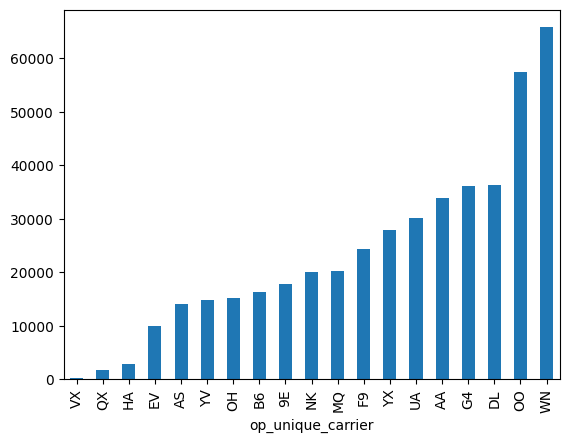
\includegraphics[width=0.45\textwidth]{fig/skew.png}
\caption{Skew Observed in the Data}
\label{fig:skew}
\end{figure}

The other reason for Spill is less partition memory. In this case Spill is caused when there is less memory available for each partition while processing data. While looking into the solutions to mitigate Spill, we found that we can manage the number of partitions that spark uses to handle the data by configuring the parameter \emph{‘spark.sql.shuffle.partitions’}. The default value for this is 200. Meaning that spark can create maximum of 200 partitions of our dataset, but it adapts according to the size of the dataset. We observed on the terminal window that for our application spark was using around 55 to 70 partitions. We realized that, since our dataset size is roughly 6GB, and if we want each partition to have minimum 256 MB of memory, we should set the numbers of partitions to 48. Thus, we configured the \emph{‘spark.sql.shuffle.partitions’} to 48.

\begin{figure}[H]
\centering
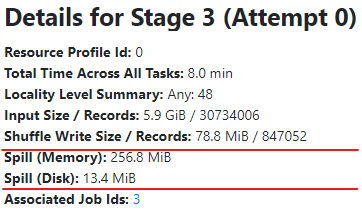
\includegraphics[width=0.35\textwidth]{fig/Spill 2.png}
\caption{Spill Observed in the Data on Spark UI}
\label{fig: spill}
\end{figure}



\subsubsection{Serialisation}
The data cleaning stage of our application originally was using UDF's which are quite slow compared to the pyspark native functions. In figure \ref{fig:fast_data_clean} the new data cleaning functions that replace the ones from figure \ref{fig:cleaning_pyspark} can be seen. These will have the exact same functionality as before but thanks to being native funtions should come with a significant performance increase. As an added bonus these functions also make the code more compact and simple to read.

\begin{figure}[H]
\centering
\begin{lstlisting}
flight_data = flight_data.na.drop(subset=['year', 'origin_airport_id', 'dest_airport_id', 'fl_date'])
flight_data = flight_data.fillna({'arr_delay_new': 0.0})
\end{lstlisting}
\caption{pyspark native data cleaning}
\label{fig:fast_data_clean}
\end{figure}

\subsubsection{Shuffle}
Our code uses 4 joins with 3 different tables so making sure that the joins are working as fast as possible is important to our use case . To do this we both tested forcing the code to use broadcast joins and sort merge joins. The broadcast versions of all the joins can be seen in figure \ref{fig:broadcast_joins} while the sort merge joins can be seen in figure \ref{fig:sortmergejoins}. The lookup tables over all we expect to be faster with a broadcast join while for the main table we are uncertain ahead of time which will be faster. Something to keep in mind is that spark will attempt to automatically choose what it believes will be the fastest join so manually forcing a specific type of join could also potentially slow the code down.

\begin{figure}[H]
\centering
\begin{lstlisting}
flight_data = flight_data.join( 
		broadcast(carriers.select('id', col('val').alias('airline')))
	, flight_data['op_unique_carrier'] == carriers['id']
	, how='left')

flight_data = flight_data.join(	
		broadcast(airports.select('id', col('val').alias('origin_airport')))
	, flight_data['origin_airport_id'] == airports['id']
	, how='left')

airports_alias = airports.alias('airports_alias')
flight_data = flight_data.join( 
    broadcast(airports_alias.select('id', col('val').alias('dest_airport')))
	, flight_data['dest_airport_id'] == airports_alias['id']
	, how='left')

flight_data = flight_data.join( 
		broadcast(carriers.select('id', col('val').alias('airline')))
	, flight_data['op_unique_carrier'] == carriers['id']
	, how='left')
\end{lstlisting}
\caption{broadcast joins}
\label{fig:broadcast_joins}
\end{figure}

\begin{figure}[H]
\centering
\begin{lstlisting}
flight_data = flight_data.sort('op_unique_carrier')
carriers = carriers.sort('id')
flight_data = flight_data.join(
		carriers.select('id', col('val').alias('airline'))
	, flight_data['op_unique_carrier'] == carriers['id']
	, how="left"
)

flight_data = flight_data.sort('origin_airport_id')
airports = airports.sort('id')
flight_data = flight_data.join(
		airports.select('id', col('val').alias('origin_airport'))
	, flight_data['origin_airport_id'] == airports['id']
	, how="left"
)

airports_alias = airports.alias('airports_alias')
flight_data = flight_data.sort('dest_airport_id')
airports_alias = airports_alias.sort('id')
flight_data = flight_data.join(
		airports_alias.select('id', col('val').alias('dest_airport'))
	, flight_data['dest_airport_id'] == airports_alias['id']
	, how="left"
)
\end{lstlisting}
\caption{sort merge joins}
\label{fig:sortmergejoins}
\end{figure}

When testing the sort merge joins to be certain that pyspark would use them over broadcast joins we also had to make the configuration changes shown in figure \ref{fig:sortmergeconfig}. With these configuration settings we could be certain that the desired joins would be used.

\begin{figure}[H]
\centering
\begin{lstlisting}
spark.sql.join.preferSortMergeJoin              true
spark.sql.adaptive.autoBroadcastJoinThreshold   -1
\end{lstlisting}
\caption{spark configurations to force a sort merge join}
\label{fig:sortmergeconfig}
\end{figure}


\section{Results}
\label{sec:results}
The results from all of our optimisations can be seen in table \ref{tab:performance}. It should be noted that each optimisation builds on top of the last one, this means that after applying an optimisation that optimisation is also present for the next optimisation in the table. The only exception to this are the two shuffle optimisations, since these are affecting the same part of the code these had to replace each other.

\begin{table}[H]
    \centering
    \begin{tabular}{c|c|c}
        Problem to solve & Optimisation & Execution time (min.)\\
        \hline
        baseline code & - & 2.4 \\
        Spill & Setting partitions to 48 & 2\\
        Serialization & Eliminating UDF's & 1.6 \\
        Shuffle 1 & Using Broadcast joins & 1.3\\
        Shuffle 2 & Using Sort Merge joins & 1.4\\
    \end{tabular}
    \caption{the optimisation results}
    \label{tab:performance}
\end{table}

With these results we can see the reducing the spill and getting rid of the UDF's had the largest performance impact. while forcing the code to use one specific type of join made a relatively smaller difference. The difference between the two types of joins is negligible and considering how short the over all run time of the program is it could be argued they are within margin of error of each other.


\section{Discussion}
\label{sec:discussion}
The observered results have shown that replacing the UDF's have the larger influence on the execution time. Reducing the allowed number of partitions to 48 also gave some improved results. While tuning the spark.sql.shuffle.partitions parameter we tested with 12, 32 and 64 partition numbers as well. Reducing it to 12 increased the execution time a bit, which seems logical since that would reduce the parallelism factor. Setting the value to 64 performed the same as it did with the default value of 200. The reason for this is our dataset size is too small and spark does self-optimization in many cases and in this case, it was only using 55-70 partitions, even when max value was set as 200. Hence, setting the value to 64 did not show any improvement. The performance for the values 32 and 48 were almost same but we chose 48 as we read that the optimal parallelism level is from 36 to 72 for a dataset with size as small as ours.\cite{tuning}

The different join techniques did not show any visible improvement in performance. One thing we observed was that Spark was automatically choosing to use broadcast join while executing the application, even when no join was explicitly mentioned. By this we concluded that explicitly mentioning join in the code had no impact on the application performance. In fact spark preferred the broadcast join so strongly for us that settings the configuration to prefer the sort merge join was not enough to get it to use it, we also had to set the broadcast join threshold to -1.

Overall it was difficult to show how much our optimisations actually mattered, this was most likely due to the dataset not being very large and the calculations being relatively simple. But if we had more data, we could experiment with different skew optimization techniques to see how they affect the performance.


\appendix
\section{Appendix}

A link to the GitHub repository with all the code can be found here: \href{https://github.com/sbthepotato/DAT500-Project-23V}{\textcolor{blue}{https://github.com/sbthepotato/DAT500-Project-23V}}


\bibliographystyle{ACM-Reference-Format}
\bibliography{bibliography}

\end{document}
